\chapter{JUDUL BAB}
\section{Section}
\lipsum[1]
Example equation:

inline equation $E=m\cdot c^2$

displayed equation

\begin{equation}
    E=m\cdot c^2
\end{equation}

\subsection{Subsection}

\begin{figure}[H]
    \centering
    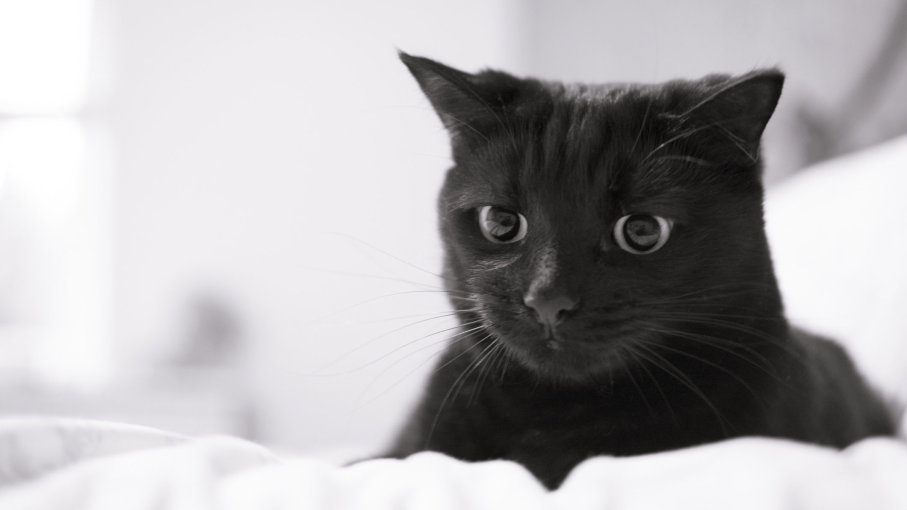
\includegraphics[width=5cm]{random-cat}
    \caption{A picture of random cat found on internet}\label{random-cat}
\end{figure}

This is an example of picture reference~\cref{random-cat}

Bibliography in IEEE style:

Newton's law of universal gravitation states that \textit{each mass particle attracts every other particle in the universe with a force that varies direcly as the product of the two masses and inversely as the square of the distance between them.}~\autocite{book:classical}

Example table:

\begin{table}[H]
    \centering
    \caption{Example table}\label{table1}
    \begin{tabular}{ccc}
        \toprule
        No & Column & Column1 \\
        \midrule
        1  & A      & B       \\
        2  & C      & D       \\
        3  & E      & F       \\
        4  & G      & H       \\
        \bottomrule
    \end{tabular}
\end{table}

This is an example of listing
\begin{lstlisting}[language=c++, caption={C++ Hello World!}, frame=shadowbox, numbers=left]
    #include <iostream>

    int main() {
        std::cout << "Hello World!";
        return 0;
    }
\end{lstlisting}

\lipsum[1]
\subsection{Subsection}
\lipsum[1]
\section{Section}
\lipsum[2]
